En este capitulo trataremos sobre los problemas que encontramos al momento de desarrollar la aplicación y asi mismo como hicimos para resolverlo.

\section{Desarrollo}
Desarrollo del Juego de Buscaminas en Android, implementado para que corra en un TABLE con una versión 3.0.
El juego comienza con la eleccion de 4 acciones:
\newline
\newline
\begin{enumerate}
	\item {Nuevo Juego}
	\item {Puntajes}	
	\item{Reglas}
	\item{Desarroladores}
\end{enumerate}
\begin{figure}[htbp]
\begin{center}
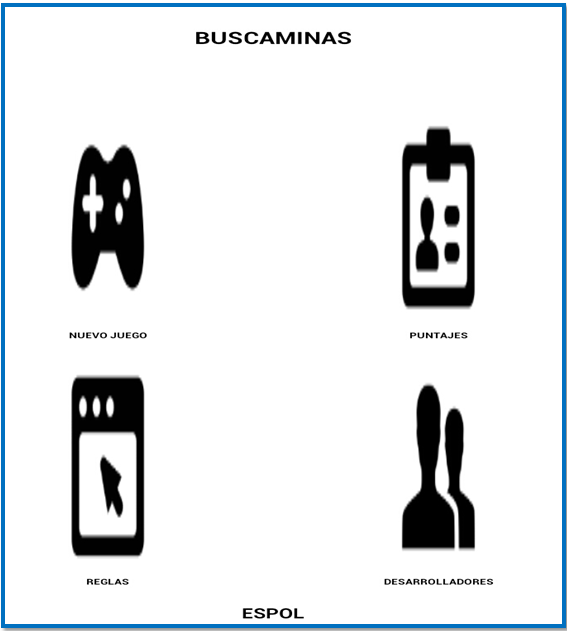
\includegraphics[width=.50\textwidth]{./imagenes/menu.png}
\caption{Menu principal}
\end{center}
Decidimos desarrollar estos botones de una manera diferente, a la convencional, decidimos poner una imagen que identifique a cada accion.
\end{figure}



\begin{figure}[htbp]
\begin{center}
\includegraphics[width=.60\textwidth]{./imagenes/niveles.png}
\caption{Niveles}
\end{center}
Una vez que ingresábamos a NUEVO JUEGO, ingresábamos a esta ventana, que podíamos ingresar el nombre del jugador, el nivel del juego y le dábamos clic en el botón Siguiente.
\end{figure}

\begin{figure}[htbp]
\begin{center}
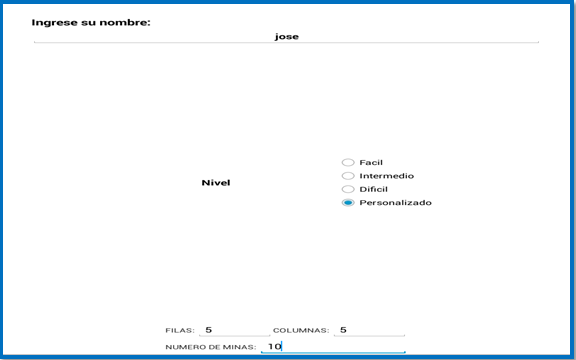
\includegraphics[width=.60\textwidth]{./imagenes/menu2.png}
\caption{Niveles}
\end{center}
deseamos jugar el nivel personalizado, nos aparecerá en la misma ventana 3 campos más; números de filas, números de columnas y el número de bombas para crear una partida personalizada.
\end{figure}
\newpage
AL momento de jugar tendremos 4 niveles:
En estas ventana comenzamos a jugar en los diferentes niveles, y debemos tratar de jugarlo en el menor tiempo posible, para poder estar entre los puntajes más altos del juego, para cada nivel.

\begin{figure}[htbp]
\begin{center}
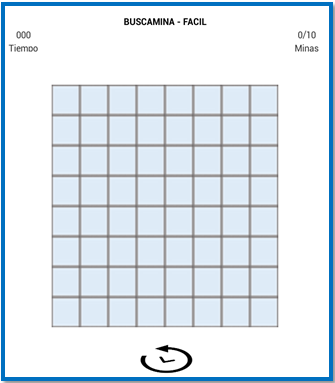
\includegraphics[width=.30\textwidth]{./imagenes/tablero2.png}
\caption{NIVEL FACIL}
\end{center}
Este nivel cuenta con 8x8 celdas, cuenta con 10 minas, también cuenta con el cronometro del tiempo en segundos y cuenta con el botón reiniciar.
\end{figure}

\begin{figure}[htbp]
\begin{center}
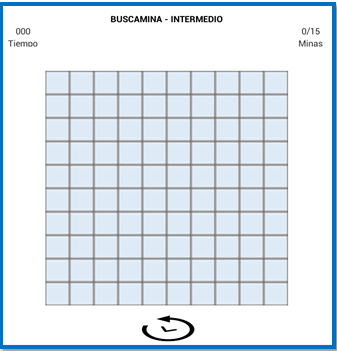
\includegraphics[width=.30\textwidth]{./imagenes/tablero3.png}
\caption{NIVEL INTERMEDIO}
\end{center}
Este nivel cuenta con 10X10 celdas, cuenta con 15 minas, también cuenta con el cronometro del tiempo en segundos y cuenta con el botón reiniciar.
\end{figure}


\begin{figure}[htbp]
\begin{center}
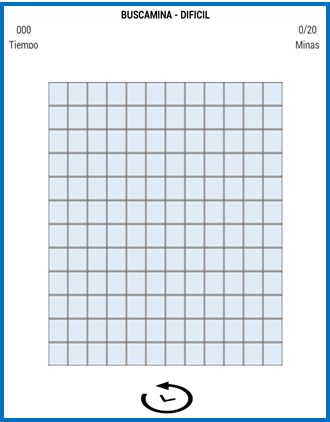
\includegraphics[width=.30\textwidth]{./imagenes/tablero4.png}
\caption{NIVEL DIFICIL}
\end{center}
Este nivel cuenta con 12X12 celdas, cuenta con 20 minas, también cuenta con el cronometro del tiempo en segundos y cuenta con el botón reiniciar.
\end{figure}


\begin{figure}[htbp]
\begin{center}
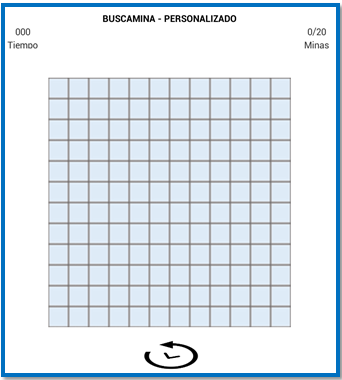
\includegraphics[width=.30\textwidth]{./imagenes/tablero5.png}
\caption{NIVEL PERSONALIZADO}
\end{center}

Este nivel cuenta con que podemos ingresar matrices desde 3x3 hasta 12x12 celdas, cuenta con minas desde 3 minas hasta 143 minas, también cuenta con el cronometro del tiempo en segundos y cuenta con el botón reiniciar.
\end{figure}


\begin{figure}[htbp]
\begin{center}
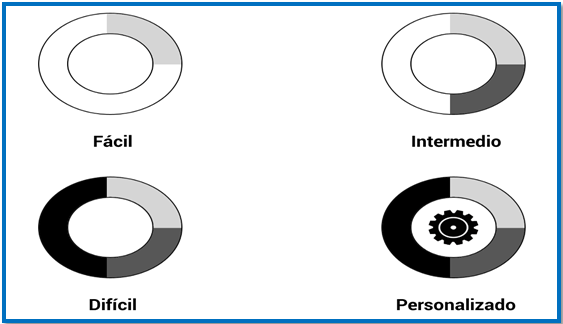
\includegraphics[width=.65\textwidth]{./imagenes/niveles2.png}
\caption{Niveles}
\end{center}

Después por recomendación del profesor, nos pidió que la ventana para elegir los niveles tenga la misma temática del Menú Principal, entras palabras que también tenga n botones que identifique cada acción.
\end{figure}

\begin{figure}[htbp]
\begin{center}
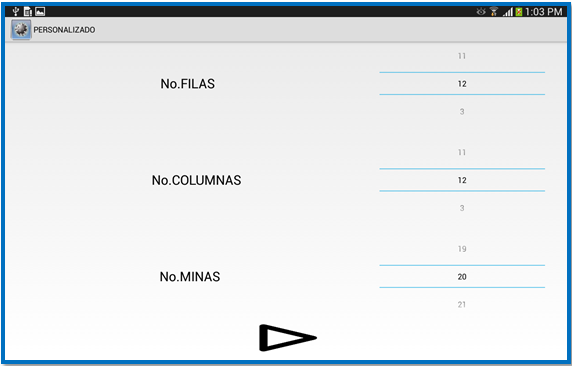
\includegraphics[width=.65\textwidth]{./imagenes/perzonalizado.png}
\caption{Nivel Perzonalizado}
\end{center}
Esta ventana aparecerá si elegimos el nivel personalizado, en donde ingresábamos en nombre y tiempo del jugador.
\end{figure}

\begin{figure}[htbp]
\begin{center}
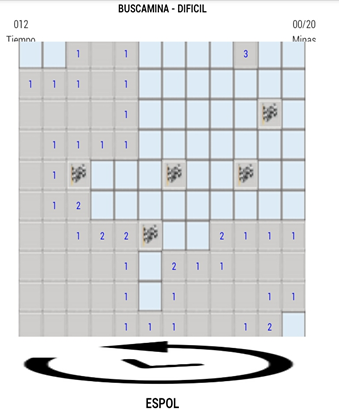
\includegraphics[width=.70\textwidth]{./imagenes/tableroBoton.png}
\caption{Tablero}
\end{center}

Cierto día creamos la bandera en el código, pero al momento de des ocultar una celda que tiene bombas, solo explota loas bombas q esta alrededor de cierta celda.
\end{figure}

\begin{figure}[htbp]
\begin{center}
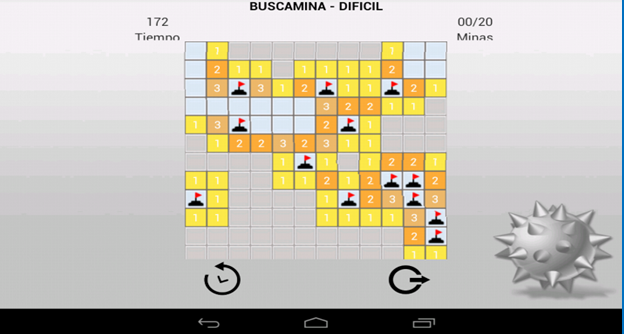
\includegraphics[width=.70\textwidth]{./imagenes/tableroCasilas.png}
\caption{TableroCasillas}
\end{center}

También implementamos que los numero que sale alrededor de otro número, salgas de diferentes colores, para que se pueda ver más colorido.
\end{figure}

\begin{figure}[htbp]
\begin{center}
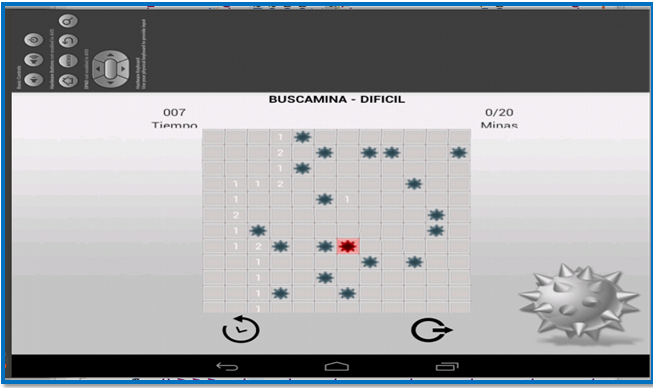
\includegraphics[width=.70\textwidth]{./imagenes/tableroBombas.png}
\caption{TableroBombas}
\end{center}
Aquí también aparecen las bombas encontradas  y la bomba estallada
\end{figure}

\begin{figure}[htbp]
\begin{center}
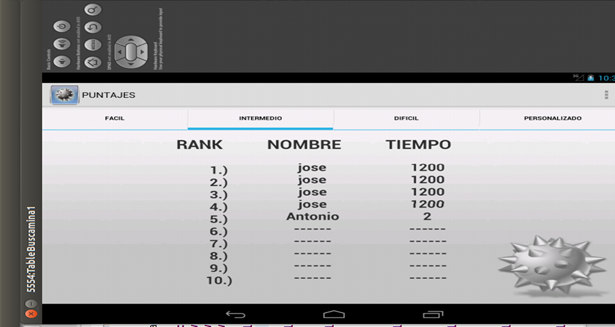
\includegraphics[width=.70\textwidth]{./imagenes/puntajes.png}
\caption{Puntajes}
\end{center}

Por último, si el jugador gana alguna partida, deberá ingresar su nombre y tiempo, y sus datos.
\end{figure}
